\section{Survival of small populations}
\label{sec:small}

Consider again the basic Galton--Watson process in which each cell leaves behind two
daughters or dies, and suppose it is near critical --- either just below or just
above. With the probability of replication $p$ and of death $1-p$ each close to a
half, a lineage dies out at its first round almost half the time. Should it pass one
generation, both of its two offspring will fail at their own first attempt with
probability around $0.25$. So the lineage of that initial cell reaches the second
generation only with likelihood approximately $0.375$:
\begin{equation*}
0.375 \approx \underbrace{(1-0.5)}_{\text{no extinction at the first step}}\times\underbrace{(1-0.5\times0.5)}_{\text{nor at the second}} .
\end{equation*}

More generally, survival to a given generation is quantified by iterating the
\pgf{}. With $\phi(z) = pz^2 + (1-p)$ from \cref{eq:pgfbinary}, the extinction and
survival probabilities follow from
\begin{equation}
\label{ext}
u_{n+1} = p\,u_n^2 + 1-p ,
\qquad
S_{n+1} = 2pS_n - pS_n^2 ,
\end{equation}
started at $u_0 = 0$, $S_0 = 1$. At exactly critical branching this gives, for
$n = 1,2,3,4$,
\begin{equation*}
u_n = 0.500,\ 0.625,\ 0.695,\ 0.741\quad(3\ \text{s.f.}),
\end{equation*}
so the likelihood of process survival decays quickly with ongoing rounds of
replication, and does so almost as fast just above criticality as just below
(\cref{fig:earlySn}).

\begin{figure}[ht]
\centering
  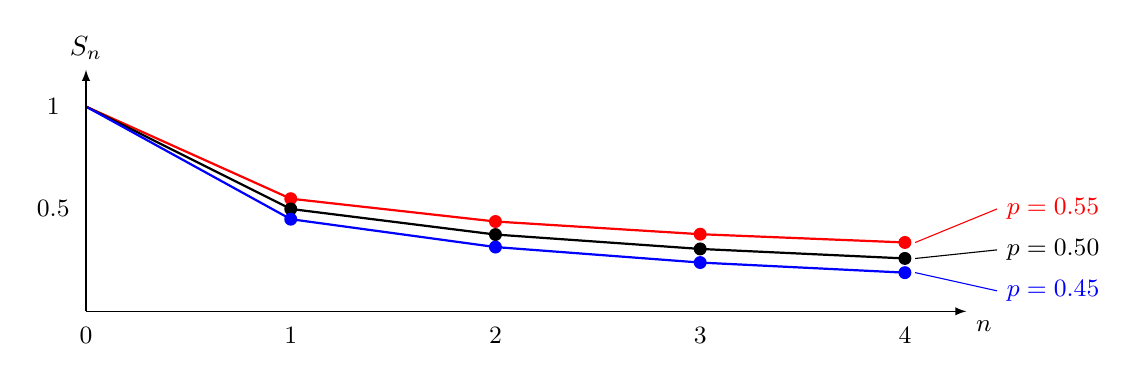
\begin{tikzpicture}[scale = 2.6]
    \foreach \x/\y/\color in {1/0.55/red, 2/0.4386250/red, 3/0.3766719/red, 4/0.336304/red,
                              1/0.5/black, 2/0.375/black, 3/0.3046875/black, 4/0.25827/black,
                              1/0.449999/blue, 2/0.313874/blue, 3/0.2381546/blue, 4/0.188816/blue}
      \fill[color=\color] (\x, \y) circle (0.9pt);
    \draw[red, thick] (0, 1) -- (1, 0.55) -- (2, 0.4386250) -- (3,0.3766719) -- (4,0.336304);
    \draw[black, thick] (0, 1)--(1,0.5) --  (2,0.375) -- (3,0.304687) -- (4,0.25827);
    \draw[blue, thick] (0, 1)--(1,0.449999)  --  (2,0.313874) -- (3,0.238154) -- (4,0.18881);
    \draw[-latex] (0,0) -- (4.3,0) node[below right, font=\small] {$n$};
    \draw[-latex] (0,0) -- (0,1.18) node[above] {$S_n$};
    \foreach \x/\lab in {0/0, 1/1, 2/2, 3/3, 4/4} \node[font=\small] at (\x, -0.12) {\lab};
    \foreach \y/\lab in {0.5/0.5, 1/1} \node[font=\small] at (-0.16, \y) {\lab};
    % leader lines from each curve end to a well-separated label
    \draw[red,  thin] (4.05,0.336) -- (4.45,0.50);
    \draw[black,thin] (4.05,0.258) -- (4.45,0.30);
    \draw[blue, thin] (4.05,0.189) -- (4.45,0.10);
    \node[red,  font=\small, anchor=west] at (4.45, 0.50) {$p=0.55$};
    \node[black,font=\small, anchor=west] at (4.45, 0.30) {$p=0.50$};
    \node[blue, font=\small, anchor=west] at (4.45, 0.10) {$p=0.45$};
  \end{tikzpicture}
\caption{Survival probability over the first four generations from a single
progenitor, from \cref{ext}. Even in the supercritical case ($p=0.55$) the early
decay is steep, and the three curves have barely separated by $n=4$. Whatever
advantage supercriticality confers, it is not an early-generation advantage.}
\label{fig:earlySn}
\end{figure}

\subsection{An initial cohort of size \texorpdfstring{$k$}{k}}
\label{sec:cohort}

Now suppose $\zz_0 = k$: the process begins not with a single unit but with a group,
small to moderate in number, perhaps $k=10$. Under supercritical branching, as the
count increases the growth becomes more predictably exponential --- a large number
of units lets the expected dynamics show through the haze of individual
stochasticity. But the founding cohort is precisely the regime in which that haze
dominates.

So for such an initial colony --- say ten pathogenic bacteria in a mammalian host
--- what are its chances of persistence, of going on to found a full-blown
infection? The question is answered by asking for the probability that at least one
descendant remains, that is, that not every one of the $k$ founding lineages has
gone extinct. Since the lineages are independent and each dies out by generation $n$
with probability ${}_1u_n$, all $k$ disappear with probability
$\bigl({}_1u_n\bigr)^k$, and so
\begin{equation}
\label{eq:Snk}
S^{(k)}_n = 1 - \bigl({}_1u_n\bigr)^{k}.
\end{equation}

\begin{figure}[ht]
\centering
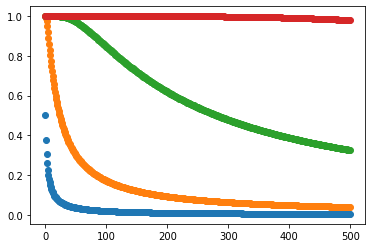
\includegraphics[width=0.56\textwidth]{figures/IMG_ch3/kvals.png}
\caption{Survival probability $S^{(k)}_n$ from \cref{eq:Snk} out to $500$
generations at exact criticality, $p=0.5$, for $k=1,10,100,1000$ (blue through to
red). A larger founding cohort buys longevity, but at criticality every curve is
still headed for zero.}
\label{fig1}
\end{figure}

\begin{figure}[ht]
\centering
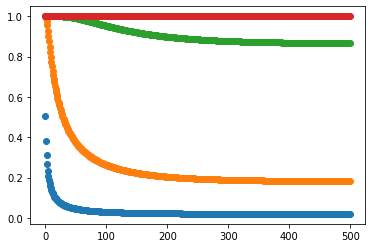
\includegraphics[width=0.45\textwidth]{figures/IMG_ch3/kvals505.png}
\hfill
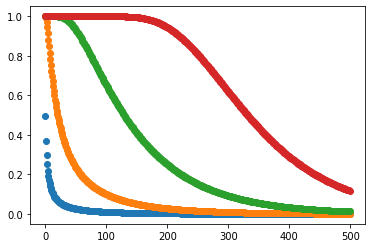
\includegraphics[width=0.45\textwidth]{figures/IMG_ch3/kvals495.png}
\caption{As \cref{fig1}, but with $p$ displaced slightly from criticality: $p=0.505$
on the left (supercritical), $p=0.495$ on the right (subcritical). The benefit of a
large initial cohort is acutely sensitive to which side of $\tfrac12$ the process
sits on; a displacement of half a percent is enough to separate curves that were
nearly coincident in \cref{fig1}.}
\label{fig2}
\end{figure}

\Cref{fig1,fig2} show $S_n^{(k)}$ through $500$ generations for $k=1$, $10$, $100$
and $1000$. The effect visible in \cref{fig1} --- that a greater first cohort gives
improved longevity --- is highly sensitive to the criticality of the process.
Persistence improves quickly as $p$ approaches $\tfrac12$ from below and continues to
improve dramatically into supercriticality; \cref{fig2} shows the same experiment
with $p$ slightly above and slightly below $\tfrac12$.

\subsection{An aside on early replication}
\label{sec:earlyrep}

It is worth noting that the same conditioning effect has been identified in a quite
different setting: the longevity and size of phylogenetic clades. Those clades that
have persisted through the ages, and which are often of superior diversity, turn out
to have experienced an above-average early rate of species origination --- an
observation drawn from the fossil record itself. Budd and Mann \cite{Budd2018} argue
that this empirical fact may be a statistical consequence rather than a biological
one: if one runs a large number of homogeneous birth--death processes and retains
only those which happen to survive to some arbitrary large positive time --- ``the
present'' --- then the retained set is automatically enriched for early rapid
origination, with no change in the underlying rates required. The apparent slowdown
in diversification that follows is then not a slowdown at all but a reversion to the
mean, an effect known as the \emph{push of the past}.

That is precisely the conditioning of \cref{sec:qsd} seen from the other side. There
we conditioned a subcritical process on survival and found that its mean settled to
$1/A(p)$ rather than decaying; here one conditions a critical-or-supercritical
process on survival to the present and finds its early growth inflated. In both
cases the conditioning, not the mechanism, does the work.

The parallel suggests a hypothesis on the pathogenic side: that it is of advantage to
an infectious agent to secure a high probability of early replication, even at some
cost to individual survival through later generations. \Cref{fig:earlySn} is the
reason to take the suggestion seriously --- the first few generations are where
nearly all of the extinction risk is concentrated.

\subsection{Discrete birth--death--catastrophe}
\label{sec:bdc}

Until the point of catastrophe, a discrete-time birth--death--catastrophe process
behaves exactly as the basic Galton--Watson model with regard to its limiting
conditional distribution. Conditioning on non-rupture, and conditioning also on
non-extinction by death, the process exhibits a stationary limiting distribution.
Whether a quasi-stationary distribution survives when one conditions on
\emph{neither} death nor catastrophe is a separate question, and one best settled by
simulation. Either way it is useful to have the probability of non-catastrophe in
hand.

\subsubsection*{Probability of rupture at step \texorpdfstring{$n$}{n}}

Let $\kappa$ be the probability that a given individual initiates catastrophe at a
step. A single individual fails to cause rupture with probability $1-\kappa$, two
with $(1-\kappa)^2$, and in general a cohort of size $N$ with $(1-\kappa)^N$.

Consider first the case of birth and catastrophe only, with no death. Then the
census of the living population at any generation is known with certainty: from a
single progenitor the population simply doubles at each step prior to catastrophe.
The process therefore comes to its abrupt halt in generation $n$ with probability
\begin{equation*}
1-(1-\kappa)^{2^{\,n-1}},
\end{equation*}
that is, one minus the probability that none of the $2^{n-1}$ individuals present
caused it.

\subsubsection*{Probability of process survival}

Along the same lines we can define, still for the no-death case, the probability
$S_n$ that the process survives to generation $n$. Survival to generation $0$ is
certain, $S_0=1$. Survival to generation $1$ requires only that the founder
replicated without rupture, $S_1 = 1-\kappa$. For persistence to step $2$ not only
must the founder divide, but so must each of its two offspring:
\begin{equation*}
S_2 = (1-\kappa)(1-\kappa)^2 .
\end{equation*}
The pattern is clear. Survival to the $n$th generation requires every prior step to
have been passed, so
\begin{equation}
\label{eq:bdcS}
S_n = \prod_{i=0}^{n-1}(1-\kappa)^{2^i} = (1-\kappa)^{\sum_{i=0}^{n-1}2^i} = (1-\kappa)^{2^n-1}.
\end{equation}

\subsubsection*{Death included}

The difficulty comes in defining $S_n$ once death is allowed, because the size of
the living population is then no longer known with certainty from one generation to
the next. The natural guess is that the probabilities somehow shake out when the
expected population is used in place of the actual one:
\begin{equation}
\label{eq:bdcguess}
S_n \overset{?}{=} (1-\kappa)^{\sum_{i=0}^{n-1}\mean{\xx_i}} .
\end{equation}
This is almost certainly not an identity, and it is worth being explicit about why.
The map $N\mapsto(1-\kappa)^N$ is convex, so by Jensen's inequality
$\mean{(1-\kappa)^{\xx_i}}\ge(1-\kappa)^{\mean{\xx_i}}$: replacing the random census
by its mean systematically underestimates the chance of getting through a step.
Nor are the steps independent, since surviving one is evidence of a smaller
population, which raises the chance of surviving the next. Both effects push the
same way, so \cref{eq:bdcguess} is better read as a lower bound than as an equality.
How tight a bound it is remains worth checking numerically.

\subsection{Continuous-time birth--death}
\label{sec:cts}

The discrete process resists a closed form for $A(p)$, as \cref{sec:Ap} will show at
length. Its continuous-time counterpart does not, and the comparison between the two
turns out to be informative, so we record the continuous-time result here.

For the simple linear birth--death process with per-capita birth rate $\lambda$ and
death rate $\mu$, started from $N$ individuals, the extinction probability is
\cite{Allen2010}
\begin{equation}
\label{eq:p0t}
p_0(t) = \begin{cases}
\lrb{\dfrac{\mu - \mu \ee^{(\mu-\lambda)t}}{\lambda - \mu \ee^{(\mu-\lambda)t}}}^{N}, & \lambda \neq \mu,\\[12pt]
\lrb{\dfrac{\lambda t}{1+\lambda t}}^{N}, & \lambda = \mu,
\end{cases}
\end{equation}
from which the survival probability is $S^{(N)}(t) = 1 - p_0(t)$.

\subsubsection*{Limiting mean conditioned on non-extinction}

The simple birth--death model has a stationary conditional mean when $\mu>\lambda$,
that is, in the subcritical case. Exactly as in \cref{sec:condmean},
\begin{equation}
\label{condit}
\mean{\xt \mid \xt > 0} = \frac{\mean{\xt}}{S^{(N)}(t)},
\end{equation}
and the late-time limit follows on applying L'H\^opital's rule. It is quicker to take
$N=1$ and compute directly. With $\mean{\xt} = \ee^{(\lambda-\mu)t}$ and
\begin{equation*}
S(t) = 1 - \lrb{\frac{\mu - \mu\ee^{(\mu-\lambda)t}}{\lambda - \mu\ee^{(\mu-\lambda)t}}}
= \frac{\lambda-\mu}{\lambda - \mu\ee^{(\mu-\lambda)t}},
\end{equation*}
\cref{condit} gives
\begin{equation*}
\mean{\xt \mid \xt > 0} = \frac{\lambda\ee^{(\lambda-\mu)t} - \mu}{\lambda-\mu}.
\end{equation*}
For $\mu>\lambda$ the exponential decays and the limiting conditional mean is a
constant,
\begin{equation}
\label{eq:ctsqsmean}
\lim_{t\to\infty}\mean{\xt \mid \xt>0} = \frac{\mu}{\mu-\lambda} = \frac{1}{1-\lambda/\mu} \;\lrb{= \frac{1}{A_{\text{c}}}}.
\end{equation}
Written in terms of the replication probability $p = \lambda/(\lambda+\mu)$, so that
$\lambda/\mu = p/(1-p)$,
\begin{equation}
\label{eq:Acts}
\frac{1}{A_{\text{c}}} = \frac{1-p}{1-2p},
\qquad\text{that is}\qquad
A_{\text{c}}(p) = \frac{1-2p}{1-p}.
\end{equation}
The subscript ``c'' marks this as the continuous-time constant, to distinguish it
from the discrete-time $A(p)$ of \cref{lateS}.

\begin{figure}[ht]
\centering
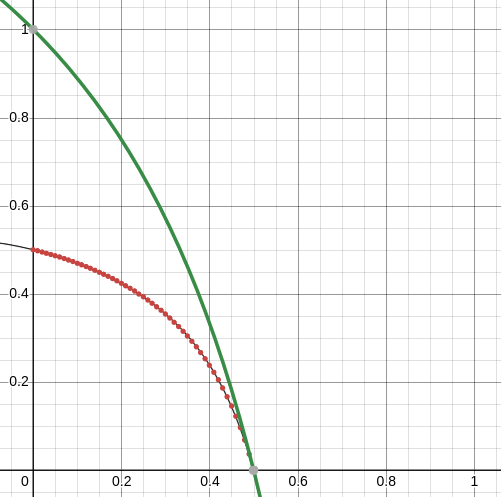
\includegraphics[width=0.5\textwidth]{figures/IMG_ch3/dtctA.png}
\caption{The continuous-time constant $A_{\text{c}}(p) = (1-2p)/(1-p)$ (green) against
high-precision numerical values of the discrete-time constant $A(p)$ (red points).
Both vanish at $p=\tfrac12$, but at $p=0$ the continuous curve starts at $1$ and the
discrete one at $\tfrac12$, and the two are not related by any constant factor in
between. The black line is a formula obtained by symbolic regression
(\cref{sec:GA}); it tracks the points closely but is not exact. \Cref{sec:compare}
accounts for the discrepancy exactly.}
\label{fig:dtct}
\end{figure}

\Cref{fig:dtct} plots $A_{\text{c}}(p)$ against numerically obtained values of the
discrete-time $A(p)$, and raises an obvious question: why does the continuous curve
start at $1$ and the discrete one at $\tfrac12$? Merely halving $A_{\text{c}}$ does not
make the two coincide, because at the other end of the range they meet. The answer
is given in \cref{sec:compare}, once the necessary machinery is in place; it turns
out that $A_{\text{c}}(p)/2$ is an exact lower bound for $A(p)$, attained only in the
limit $p\to0$.

\FloatBarrier
